\documentclass[a4paper,11pt]{report}

%
%--------------------   start of the 'preamble'
%
\usepackage[utf8]{inputenc}
\usepackage[pdftex]{hyperref}
\usepackage{titlepic}
\usepackage{color}
\usepackage{graphicx}
\usepackage{amsmath}
\usepackage[french,english]{babel}
\usepackage[pdftex]{hyperref}


% Pour les listes
\frenchbsetup{StandardLists=true}
\usepackage{enumitem}
\usepackage{amssymb}

\usepackage{fullpage}
\setlength{\topmargin}{0pt} % Pas de marge en haut
%\setlength{\oddsidemargin}{0pt} % Marge gauche sur pages impaires
%\setlength{\evensidemargin}{0pt} % Marge gauche sur pages paires


\definecolor{violeticc}{rgb}{0.6549,0,0.4588}

\hypersetup{
colorlinks=true,%
plainpages=false,%
hypertexnames=false,%
urlcolor=violeticc,%
linkcolor=violeticc%
}



%
%---------------------   end of the 'preamble'
%

%
%--------------------   PDF info
%
\pdfinfo{%
  /Title    (Installation de GeOxygene pour les développeurs)
  /Author   (Julien Perret)
  /Creator  (Julien Perret)
  /Producer (Laboratoire COGIT, IGN)
  /Subject  (Installation GeOxygene)
  /Keywords (GeOxygene, Eclipse, Java, Maven, Subversion)
}
%
%---------------------   end of the 'preamble'
%

%
%--------------------   début du report
%
\begin{document}
\selectlanguage{french}

%-----------------------------------------------------------
\title{Guide d'installation pour les développeurs}
\author{Laboratoire COGIT - IGN}
\date{\today}


\titlepic{
\includegraphics[width=0.5\textwidth]{../../resources/images/geoxygene-logo.png}}

\maketitle

%-----------------------------------------------------------
%-----------------------------------------------------------
%--  Historique des révisions
%-----------------------------------------------------------

\begin{center}

\textsc{\Large Historique des révisions}\\[0.5cm]

\bigskip
\bigskip
\bigskip

\begin{tabular}[!t]{|l||l|l|l|}
\hline
\textbf{Version}&\textbf{Date}&\textbf{Auteur}&\textbf{Version de GeOxygene}\\
\hline
\hline
1&17 mai 2010&Julien Perret&Version 1.4\\
2&31 mai 2010&Julien Perret&Version 1.4\\
3&13 janvier 2011&Cécile Duch\^ene&Version 1.4\\
4&14 janvier 2011&Julien Perret&Version 1.4\\
DRAFT&\today&Marie-Dominique Van Damme&Version 1.5\\
\hline
\end{tabular} 

\end{center}

%-----------------------------------------------------------

%-----------------------------------------------------------
%-- Tables des matières
\tableofcontents
%-----------------------------------------------------------


\chapter{Introduction}

Ce document a pour objectif de guider l'utilisateur dans son installation de la plateforme GeOxygene sous Windows ou sous Linux. On décrira d'abord l'installation des outils nécessaires, puis dans un second temps nous préciserons les démarches d'import et de compilation du code source. 

\bigskip

\noindent
Ce guide s'adresse principalement aux développeurs qui souhaitent faire leurs premiers pas dans GeOxygene.

\bigskip
\noindent
Il est à noter que la procédure d'installation et de configuration expliquée ici se base sur la version 1.5 de GeOxygene.

%-----------------------------------------------------------
\bigskip

\begin{flushleft}
    \bf
    Prérequis
\end{flushleft}

\noindent
GeOxygene est un projet Open Source écrit en JAVA. Pour pouvoir fonctionner, GeOxygene nécessite donc l'installation d'une version 6 (ou supérieure) d'une JDK. Il est possible de télécharger cet environnement sur le site de Sun à l'adresse suivante :

\bigskip

\begin{center}
\href{http://www.oracle.com/technetwork/java/javase/downloads/index.html}{http://www.oracle.com/technetwork/java/javase/downloads/index.html}
\end{center}

%-----------------------------------------------------------------------
% Installation : Eclipse
% 
%-----------------------------------------------------------------------
\chapter{Installation des outils}

%-----------------------------------------------------------------------
\section{Eclipse}

L'environnement de développement utilisé est celui d'Eclipse\footnote{http://www.eclipse.org/}, éditeur très largement utilisé aujourd'hui pour les développements JAVA.

\medskip

\subsection{Téléchargement}
Vous pouvez télécharger Eclipse sur le 
\href{http://www.eclipse.org/downloads/}{site de téléchargement d'Eclipse}. A priori, toutes les versions destinées au développement Java devraient fonctionner. Néanmoins, seules les versions Helios(3.6), Indigo(3.7), Juno (4.2), Kepler (4.3) ont été testées dans le cadre de cette documentation. Le téléchargement de cette dernière version d'Eclipse pour les différentes plate-formes est directement accessible ici~:\\

\begin{center}
\begin{tabular}[!t]{lll}
Windows&
\href{http://www.eclipse.org/downloads/download.php?file=/technology/epp/downloads/release/kepler/R/eclipse-standard-kepler-R-win32.zip}{32bit}&
\href{http://www.eclipse.org/downloads/download.php?file=/technology/epp/downloads/release/kepler/R/eclipse-standard-kepler-R-win32-x86_64.zip}{64bit}\\
Mac OS X(Cocoa)&
\href{http://www.eclipse.org/downloads/download.php?file=/technology/epp/downloads/release/kepler/R/eclipse-standard-kepler-R-macosx-cocoa.tar.gz}{32bit}&
\href{http://www.eclipse.org/downloads/download.php?file=/technology/epp/downloads/release/kepler/R/eclipse-standard-kepler-R-macosx-cocoa-x86_64.tar.gz}{64bit}\\
Linux&
\href{http://www.eclipse.org/downloads/download.php?file=/technology/epp/downloads/release/kepler/R/eclipse-standard-kepler-R-linux-gtk.tar.gz}{32bit}&
\href{http://www.eclipse.org/downloads/download.php?file=/technology/epp/downloads/release/kepler/R/eclipse-standard-kepler-R-linux-gtk-x86_64.tar.gz}{64bit}\\
\end{tabular}
\end{center}

\medskip

\subsection{Installation}
Pour installer Eclipse, il suffit de décompresser le fichier téléchargé. 

\bigskip

\noindent
Lancer Eclipse :
\begin{itemize}
\item Sous windows cela crée un répertoire nommé "eclipse", exécuter le fichier eclipse.exe
\item Sous linux cela crée un répertoire nommé "/opt/eclipse", exécuter ./eclipse
\end{itemize}

\noindent
Lors du premier lancement, une boite de dialogue vous demandera de sélectionner le répertoire racine de vos projets Eclipse. Soit vous sélectionnez celui proposé, auquel cas il sera créé ou, vous pouvez en choisir un autre.

\newpage


%--------------------------------------------------------------------------
\subsection{Proxy}

Pour installer des mises à jour, de nouveaux plugins ou des extensions, il faut qu'Eclipse puisse accèder au net pour pouvoir les télécharger.  Si vous êtes derrière un proxy, il vous faut configurer Eclipse afin qu'il en tienne compte.

\bigskip

\begin{itemize}[leftmargin=* ,parsep=0cm,itemsep=0cm,topsep=0cm]

\item Pour ce faire, accéder au menu \emph{Window/Preferences/General/Network~Connection}. Vous pouvez alors séléctionner \emph{Manual} comme \emph{Active Provider} 

\begin{center}
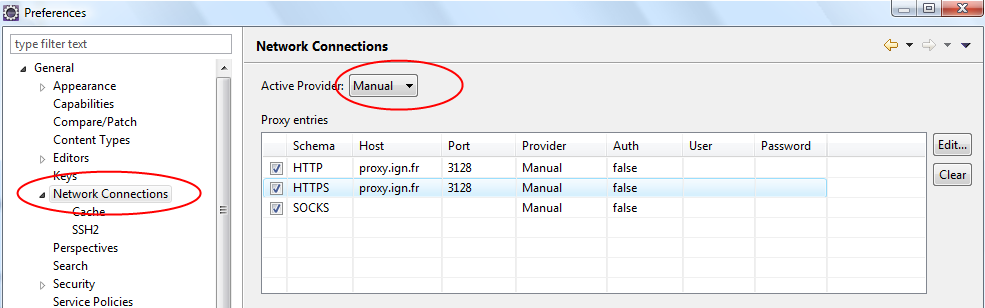
\includegraphics[width=0.8\linewidth]{proxy3}
\end{center}

\item Selectionner “HTTP” dans la liste des entrées et cliquer sur le bouton “Edit”

\begin{center}
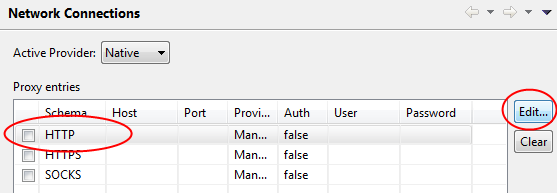
\includegraphics[width=0.5\linewidth]{proxy4}
\end{center}


\item Entrer les coordonnées de votre proxy. Pour l'IGN par exemple, il s'agit de \emph{proxy.ign.fr} avec le port \emph{3128}. Ne remplisser pas les champs d'authentification.

\begin{center}
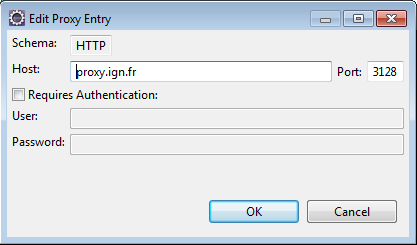
\includegraphics[width=0.4\linewidth]{proxy1}
\end{center}


\item Faire de même pour “HTTPS”

\begin{center}
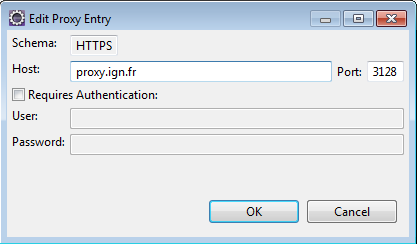
\includegraphics[width=0.4\linewidth]{proxy2}
\end{center}


\end{itemize}

%--------------------------------------------------------------------------

\subsection{Encodage}

Tous les modules de GeOxygène doivent être encodés en UTF-8. \\

\noindent
Pour ce faire, dans Eclipse :

Aller dans "Preferences $\Rightarrow$ Workspace $\Rightarrow$ Text file encoding $\Rightarrow$ Other"  et choisir UTF-8. 

\bigskip
\bigskip

%--------------------------------------------------------------------------


\noindent
Maintenant, Eclipse est prêt pour l'installation des plugins nécessaires à GeOxygene. Vous aurez besoin des plugins Maven (m2eclipse) et subversion (subclipse). Pour des questions de d\'ependance, il est pr\'ef\'erable de commencer par installer subclipse.


%-----------------------------------------------------------------------
% Installation : Subeclipse
% 
%-----------------------------------------------------------------------
%\newpage

%-----------------------------------------------------------------------
\section{Installation du plugin Subclipse dans Eclipse}

Subclipse est un plug-in Eclipse vous permettant d'utiliser Subversion (SVN) directement depuis votre \'editeur pr\'ef\'er\'e.

\begin{itemize}[leftmargin=* ,parsep=0cm,itemsep=0cm,topsep=0cm]

\medskip

\item Etape 1 : Commencer par cliquer dans le menu d’Eclipse sur l'onglet « Help », puis sur « Install New Software ».
\begin{center}
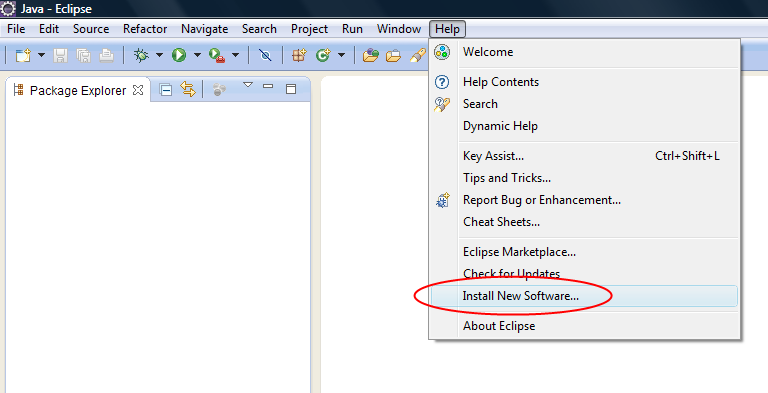
\includegraphics[width=0.4\linewidth]{../../resources/images/guide_installation/pluginInstall.png}
\end{center}

\item Etape 2 : Cliquer sur « Add » afin d’ajouter le site de subeclipse dans la liste des sites de logiciels disponibles
\begin{center}
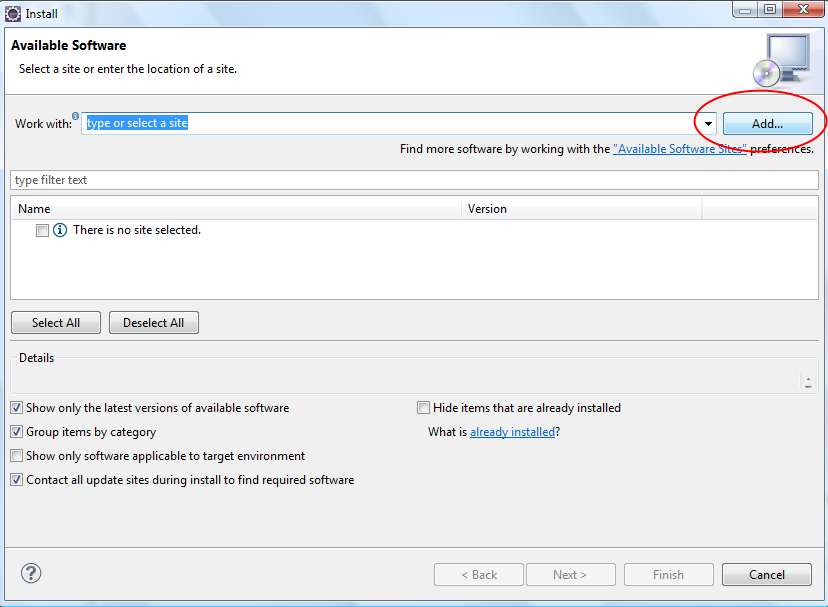
\includegraphics[width=0.4\linewidth]{../../resources/images/guide_installation/pluginNewUrl.png}
\end{center}

\item Etape 3 : Saisir dans la boite de dialogue les informations d\'ecrites ci-dessous puis cliquer sur "OK"\\

\begin{tabular}[!t]{ll}
{\bf Name : }&{Subclispe}\\
{\bf Location : }&{\href{http://subclipse.tigris.org/update_1.8.x}{http://subclipse.tigris.org/update\_1.8.x}}\\
\end{tabular}\\
\smallskip
\begin{center}
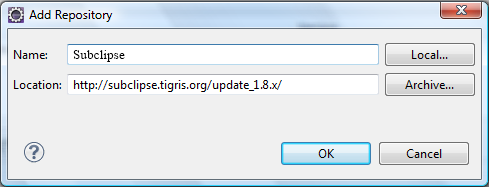
\includegraphics[width=0.4\linewidth]{../../resources/images/guide_installation/subeclipseUrl.png}
\end{center}

\newpage

\item Etape 4 : La boite de dialogue "install" affiche l'ensemble des plugins disponibles. Tout n’est pas utile, mais cocher au moins les packages marqu\'es required ainsi que SVNKit puis cliquer sur "Next".
\begin{center}
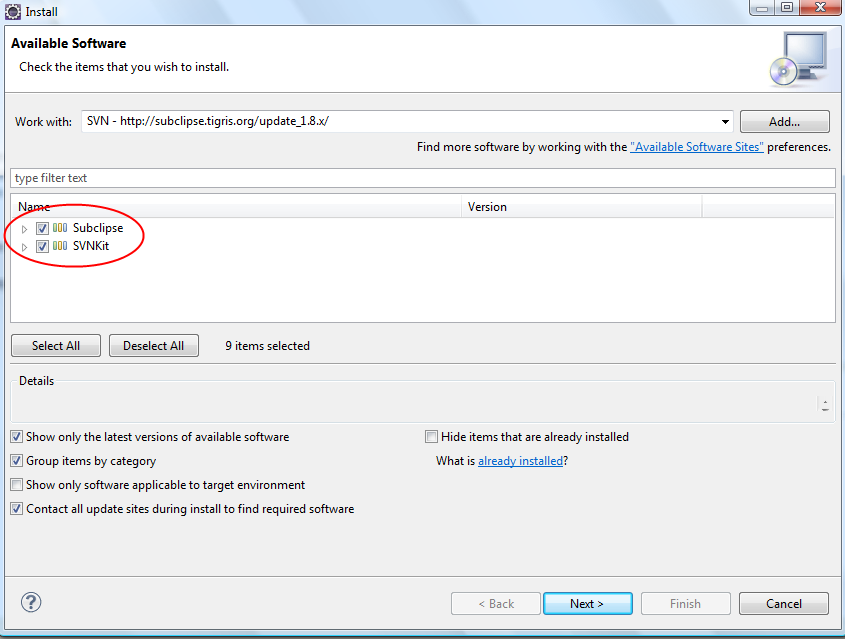
\includegraphics[width=0.4\linewidth]{../../resources/images/guide_installation/subeclipseEtape1.png}
\end{center}

\item Etape 5 : Sur la page "Install Details" cliquer juste sur le bouton "Next"
\begin{center}
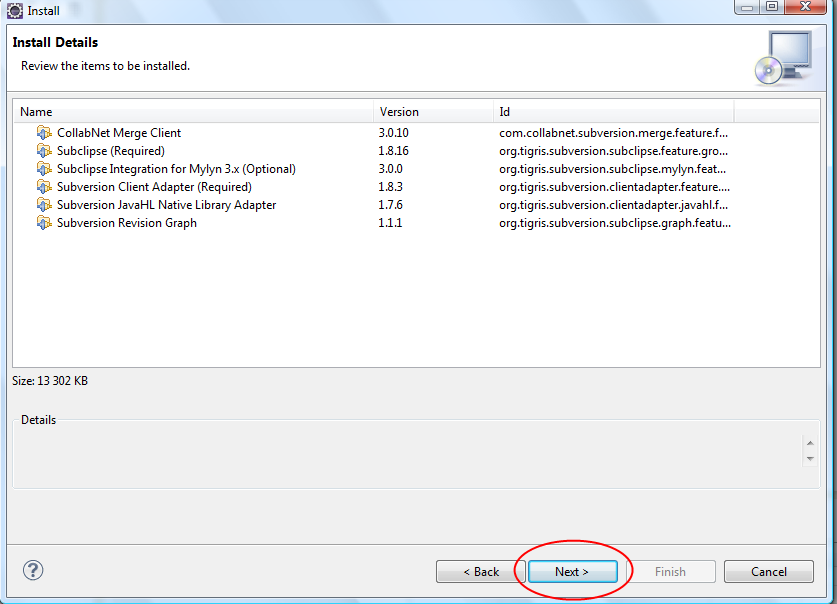
\includegraphics[width=0.4\linewidth]{../../resources/images/guide_installation/subeclipseEtape2.png}
\end{center}

\item Etape 6 : Accepter les termes de la licence de subeclipse sur la page "Review Licences" et cliquer sur "Finish" pour commencer l'installation.
\begin{center}
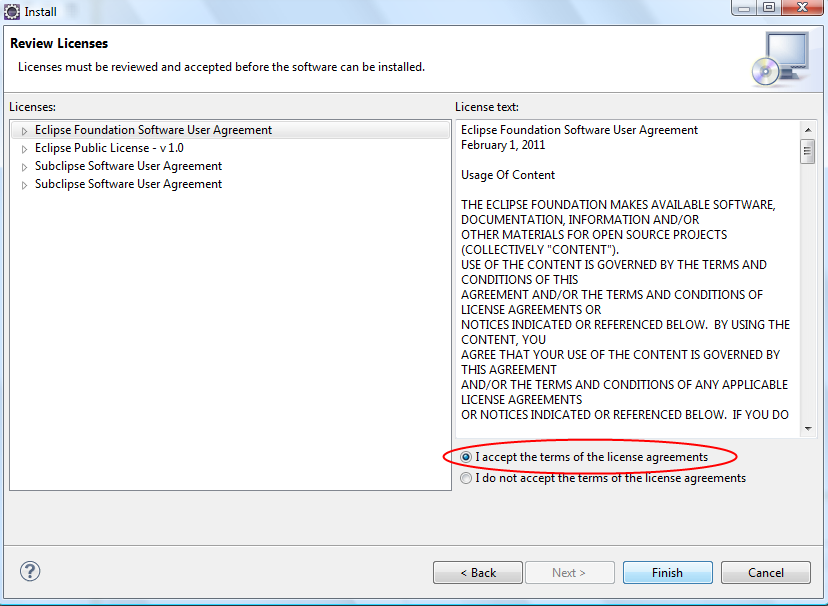
\includegraphics[width=0.4\linewidth]{../../resources/images/guide_installation/subeclipseEtape3.png}
\end{center}

\item Etape 7 : Vous allez recevoir un message d'alerte "Security Warning" parce que les jars de subeclipse ne sont pas sign\'es. Cliquer sur "OK" pour continuer l'installation.
\begin{center}
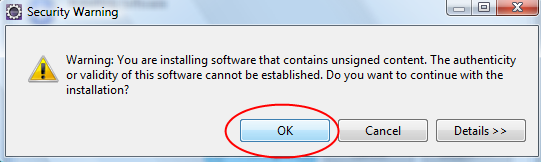
\includegraphics[width=0.4\linewidth]{../../resources/images/guide_installation/pluginNonSigne.png}
\end{center}

\newpage

\item Etape 8 : Une fois l'installation termin\'ee, pr\'ef\'erer "Restart Now" dans la prochaine boite de dialogue. 
\begin{center}
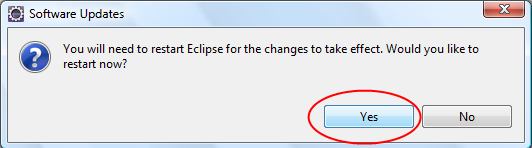
\includegraphics[width=0.4\linewidth]{../../resources/images/guide_installation/pluginRestart.png}
\end{center}
Le plugin subeclipse sera op\'erationnel après le red\'emarrage d'Eclipse.

\bigskip

\item Etape 9 : Une fois le plugin install\'e, configurer dans Eclipse l'interface SVNKit. En effet, celle-ci semble mieux fonctionner que celle par d\'efaut (JavaHL). Pour cela, dans le menu d'Eclipse Window/Preferences/Team/SVN, s\'electionner l’interface SVN "SVNKit".
\begin{center}
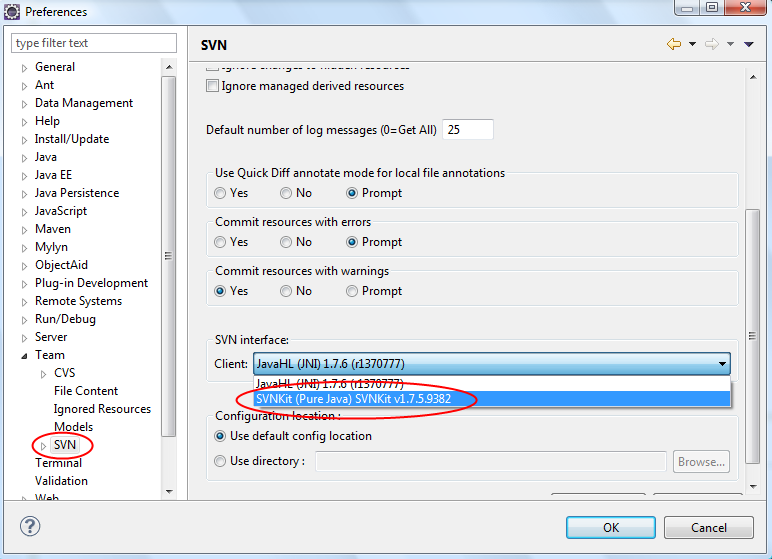
\includegraphics[width=0.4\linewidth]{../../resources/images/guide_installation/subeclipseInterface.png}
\end{center}


\end{itemize}
%-----------------------------------------------------------------------
% Installation : M2eclipse
% 
%-----------------------------------------------------------------------

%-----------------------------------------------------------------------
\section{Installation du plugin M2eclipse dans Eclipse}

GeOxygene est généré à partir de Maven\footnote{http://maven.apache.org/}.  Le projet m2eclipse fournit un support afin d'utiliser les fonctionnalités de Maven dans l'éditeur Eclipse.

\medskip

\noindent
L'intégration Maven pour Eclipse est séparée en deux plugins : le core et un module optionnel contenant des composants supplémentaires. Pour installer GeOxygene, il faut les deux.


\subsection{m2eclipse Core Components}
Reprenez les 8 premières étapes de l'installation du plugin subeclipse mais en adaptant les paramètres.

\medskip

\noindent
1. A l'étape 3 saisir :\\

\begin{tabular}[!t]{ll}
{\bf Name : }&{m2eclipse}\\
{\bf Location : }&{\href{http://m2eclipse.sonatype.org/sites/m2e}{http://m2eclipse.sonatype.org/sites/m2e}}\\
\end{tabular}\\

\smallskip
\begin{center}
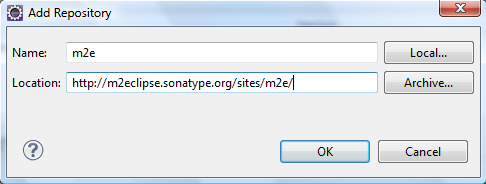
\includegraphics[width=0.4\linewidth]{../../resources/images/guide_installation/m2eclipseUrl.png}
\end{center}

\noindent
2. A l'étape 4 choisir l'unique composant "Maven Integration for Eclipse".\\
\begin{center}
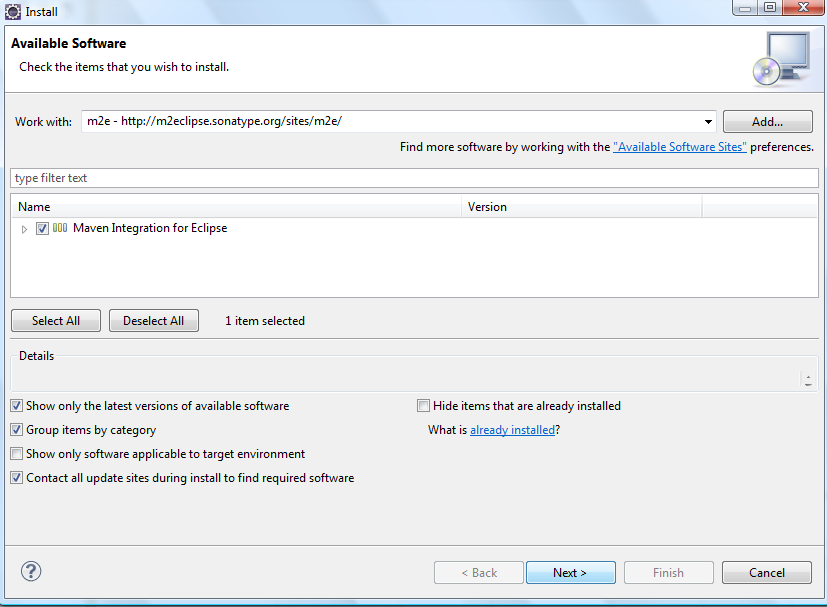
\includegraphics[width=0.4\linewidth]{../../resources/images/guide_installation/m2eclipseEtape1.png}
\end{center}

\noindent
3. A l'étape 8, une fois l'installation terminée, une fenêtre propose de redémarrer Eclipse, inutile de le faire à ce stade.




%-----------------------------------------------------------------------
%\newpage

\subsection{m2eclipse Extras}
Une dès options disponibles dans ce plugin est la possibilité d'importer directement d'un dépôt SVN un projet Maven. C'est celui que l'on va installer.

\medskip

\noindent
Reprenez une nouvelle fois les 8 premières étapes de l'installation du plugin subeclipse mais en adaptant les paramètres.

\newpage

\noindent
1. A l'étape 3 saisir :\\

\begin{tabular}[!t]{ll}
{\bf Name : }&{m2e-extras}\\
{\bf Location : }&{\href{http://m2eclipse.sonatype.org/sites/m2e-extras}{http://m2eclipse.sonatype.org/sites/m2e-extras}}\\
\end{tabular}\\

\smallskip
\begin{center}
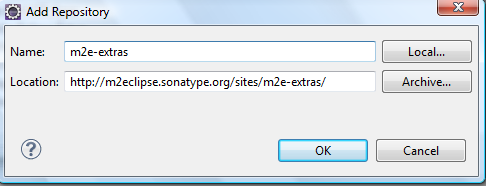
\includegraphics[width=0.4\linewidth]{../../resources/images/guide_installation/m2eclipseExtrasUrl.png}
\end{center}

\noindent
2. A l'étape 4 sélectionner au moins le composant "Maven SCM handler for Subclipse".\\
\begin{center}
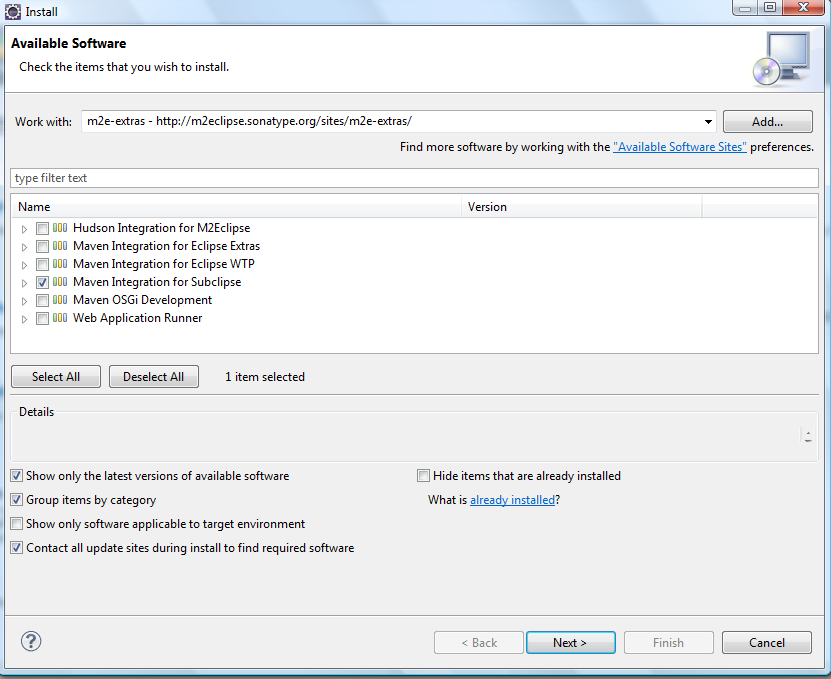
\includegraphics[width=0.4\linewidth]{../../resources/images/guide_installation/m2eclipseExtrasEtape1.png}
\end{center}

\noindent
3. A l'étape 8, une fois l'installation terminée, une fenêtre propose de redémarrer Eclipse, à ce stade il est vivement conseillé de le faire.






%-----------------------------------------------------------------------
% Installation : M2eclipse
% 
%-----------------------------------------------------------------------

%-----------------------------------------------------------------------
\section{Configuration}
Pour pouvoir utiliser toutes les fonctionalités de Maven sous Eclipse, deux étapes de configuration sont nécessaires.

\subsection{Configuration d'Eclipse}
Il faut configurer Eclipse pour s'exécuter avec un JDK et non un JRE sinon ce message d'erreur pourrait s'afficher : 

\begin{center}
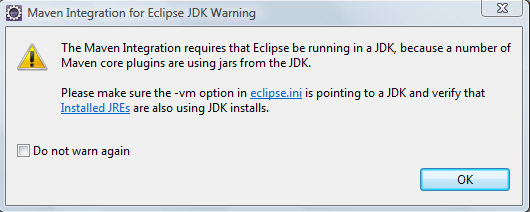
\includegraphics[width=0.4\linewidth]{warningJRE}
\end{center}

\noindent
Pour ce faire, il faut éditer le fichier \emph{eclipse.ini} situé à la racine du répertoire d'Eclipse. Rajoutez les lignes suivantes au début du fichier~:\\

\smallskip 

\begin{tabular}[!t]{l|l}
sous Linux&sous Windows\\
\verb|-vm|&\verb|-vm|\\
\verb|<jdkXXXX>/bin/java|&\verb|<jdkXXXX>\bin\javaw.exe|\\
\end{tabular}\\

\medskip 
\noindent
Où \verb|<jdkXXX>| désigne le répertoire du jdk que vous voulez utiliser, par exemple \\
\verb|c:\MesProgrammes\java\java_EE_5_SDK_Update_7\SDK\jdk|
(pour conna\^itre la valeur par défaut, vous pouvez regarder la valeur de la variable d'environnement JAVA\_HOME).

\medskip 
\begin{center}
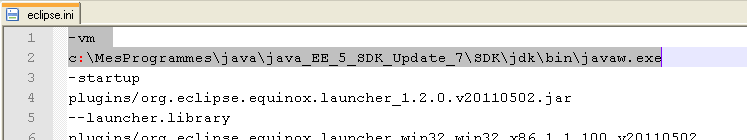
\includegraphics[width=1.0\linewidth]{eclipse_ini}
\end{center}

\medskip 
\noindent
N'ESSAYEZ PAS d'utiliser \%JAVA\_HOME\% dans le eclipse.ini, ce n'est pas pris en charge.


%----------------------------------------------------------------------------------------------------------
\subsection{Configuration de Maven}
Si vous \^etes derrière un proxy, la dernière étape consiste à configurer Maven pour utiliser le proxy. Pour ce, il faut ajouter un fichier \emph{settings.xml} dans la racine de Maven. Ce répertoire est situé à l'endroit suivant~:\\

\smallskip 

\begin{tabular}[!t]{ll}
sous Linux&\verb|~/.m2|\\
sous Windows&\verb|C:\Documents and Settings\%USER%\.m2|
\end{tabular}\\

\bigskip 

\noindent
Voici un exemple de fichier settings que vous pouvez utiliser à l'IGN~:
\begin{scriptsize}
\begin{verbatim}
<settings xmlns="http://maven.apache.org/SETTINGS/1.0.0"
  xmlns:xsi="http://www.w3.org/2001/XMLSchema-instance"
  xsi:schemaLocation="http://maven.apache.org/SETTINGS/1.0.0
                      http://maven.apache.org/xsd/settings-1.0.0.xsd">
  <interactiveMode>true</interactiveMode>
  <usePluginRegistry>false</usePluginRegistry>
  <offline>false</offline>
  <proxies>
    <proxy>
      <active>true</active>
      <port>3128</port>
      <host>proxy.ign.fr</host>
      <nonProxyHosts>localhost</nonProxyHosts>
    </proxy>
  </proxies>
  <profiles>
    <profile>
      <id>cogit</id>
      <activation>
        <activeByDefault>true</activeByDefault>
      </activation>
      <repositories>
        <repository>
          <id>central</id>
          <name>Central Maven Repository</name>
          <url>http://repo2.maven.org/maven2</url>
        </repository>
        <repository>
          <id>releases</id>
          <name>Nexus Releases Repository</name>
          <url>https://dionysos2.ign.fr/nexus-webapp-1.4.1/content/repositories/releases/</url>
        </repository>
      </repositories>
    </profile>
  </profiles>
  <activeProfiles>
    <activeProfile>cogit</activeProfile>
  </activeProfiles>
</settings>
\end{verbatim}
\end{scriptsize}





%-----------------------------------------------------------------------
%  Installation de GeOxygene
%

\chapter{Installation de GeOxygene}


%---------------------------------------------------------------------------------
Vous avez maintenant tout ce qu'il faut pour télécharger, gérer, compiler et exécuter GeOxygene.


%---------------------------------------------------------------------------------
\section{Importer le projet GeOxygene}
Dans Eclipse la création d'un nouveau projet s'effectue via l'assistant "nouveau projet". Celui-ci offre en effet une pléthore de modèles. Il suffit donc pour importer GeOxygene de choisir celui qui va extraire un projet Maven depuis un SCM (dans notre cas SVN). 

\medskip

\noindent
Comme décrits dans les deux captures d’écran ci-dessous, cliquer :

\def\imagetop#1{\vtop{\null\hbox{#1}}}
\begin{center}
\begin{tabular}[h]{c|c}        
  {d'abord sur : \emph{File} $\Rightarrow$ \emph{New}  $\Rightarrow$ \emph{Other}}& 
  {puis sur : \emph{Maven}  $\Rightarrow$ \emph{Checkout~Maven~Projects~from~SCM}} \\        
  
  \imagetop{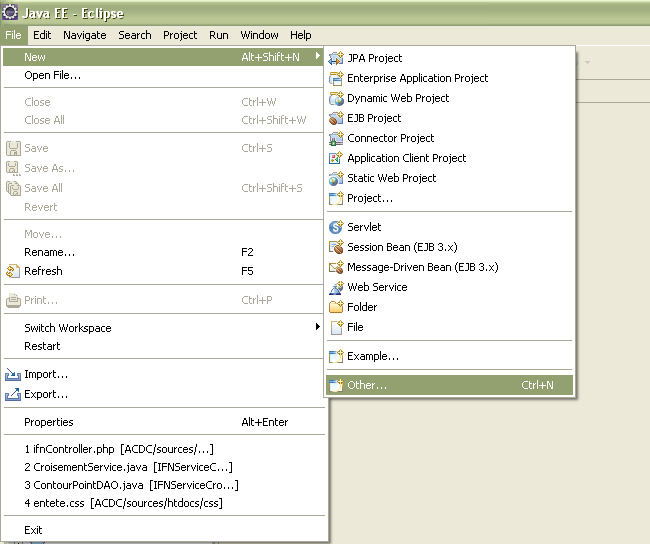
\includegraphics[width=0.39\textwidth]{../../resources/images/guide_installation/geoxygeneEtape1.png}}&
  \imagetop{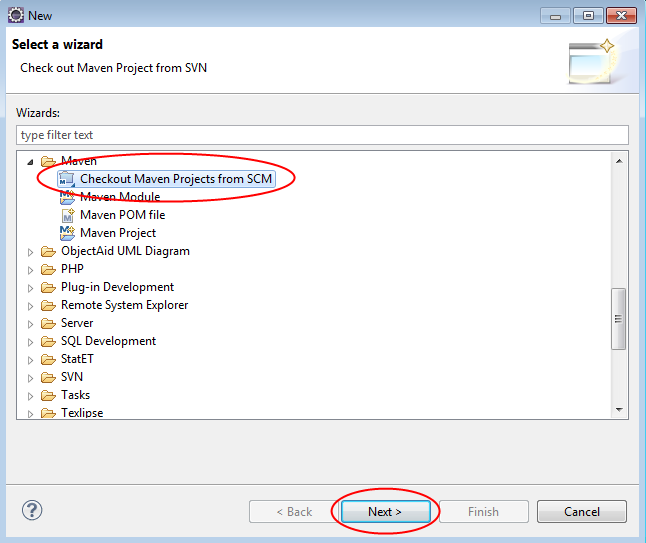
\includegraphics[width=0.61\textwidth]{../../resources/images/guide_installation/geoxygeneEtape2.png}}
\end{tabular}
\end{center}

\newpage

\noindent
Ensuite comme l'indique la figure suivante, sélectionner \emph{svn} dans la première liste comme SCM URL et indiquer l'adresse du svn de GeOxygene~:\\
\href{https://oxygene-project.svn.sourceforge.net/svnroot/oxygene-project/main/trunk/geoxygene}{https://oxygene-project.svn.sourceforge.net/svnroot/oxygene-project/main/trunk/geoxygene}, 

\begin{center}
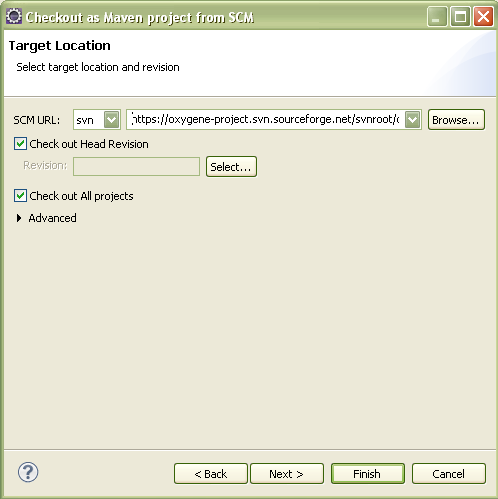
\includegraphics[width=0.5\linewidth]{../../resources/images/guide_installation/geoxygeneEtape3.png}
\end{center}

\bigskip

\noindent
puis cliquer sur "Next".

\bigskip

\noindent
Dans le panneau suivant, vous pouvez:
\begin{itemize}[label=--, leftmargin=* ,parsep=0cm,itemsep=0cm,topsep=0cm]
\item sélectionner le répertoire où sera stocké votre projet (par défaut dans le workspace courant), 
\item ajouter le projet à un working set (c'est à dire un groupe de projets)
\item modifier le nom du (ou des) projet(s) récupéré (s) (dans Advanced). Cette dernière option est utile si vous avez déjà des projets portant des noms identiques ou similaires ou si vous souhaitez ajouter à tous les projets récupérés un préfixe, un suffixe, ou utiliser un template de nom comme [groupId].[artifactId]-[version] qui vous créera, pour geoxygene, un projet nommé \emph{fr.ign.cogit.geoxygene-1.5}.
\end{itemize}

\begin{center}
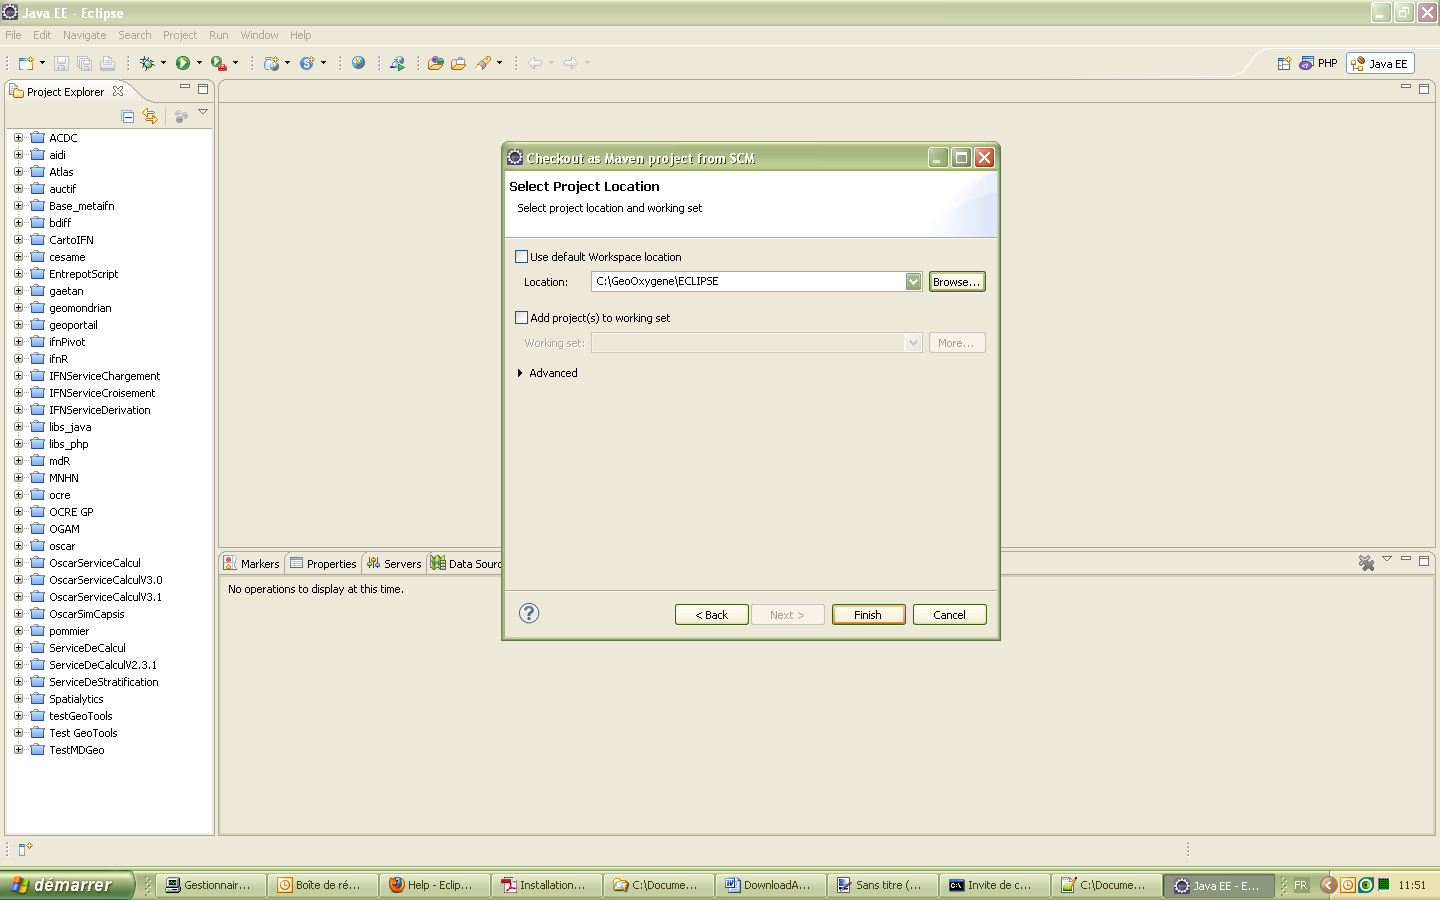
\includegraphics[width=0.5\linewidth]{../../resources/images/guide_installation/geoxygeneEtape4.png}
\end{center}

\bigskip

\noindent
Cliquez ensuite sur Finish.


%---------------------------------------------------------------------------------
\newpage
\section{Compilation}

%-------- cas 1
\begin{flushleft}
    \bf
    1er cas : vous utilisez l'option de compilation automatique
\end{flushleft}

\begin{center}
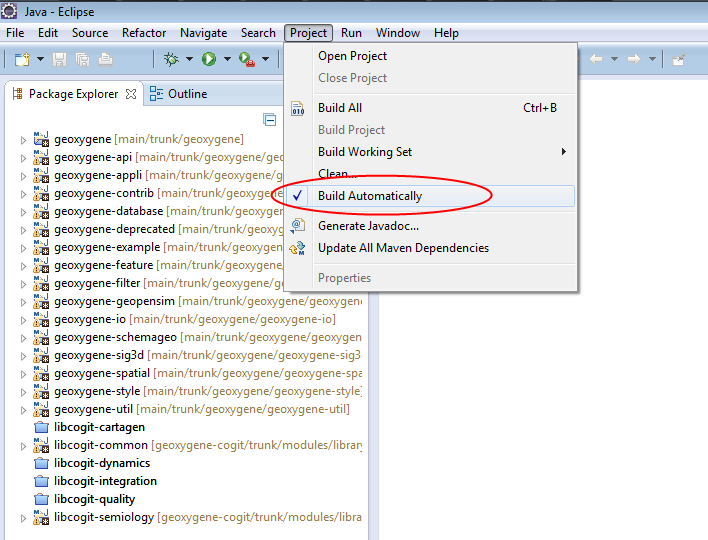
\includegraphics[width=0.5\linewidth]{../../resources/images/guide_installation/geoxygeneBuildAutomatically.png}
\end{center}

\noindent
Vous n'avez rien à faire, la compilation se lance automatiquement

%\begin{center}
%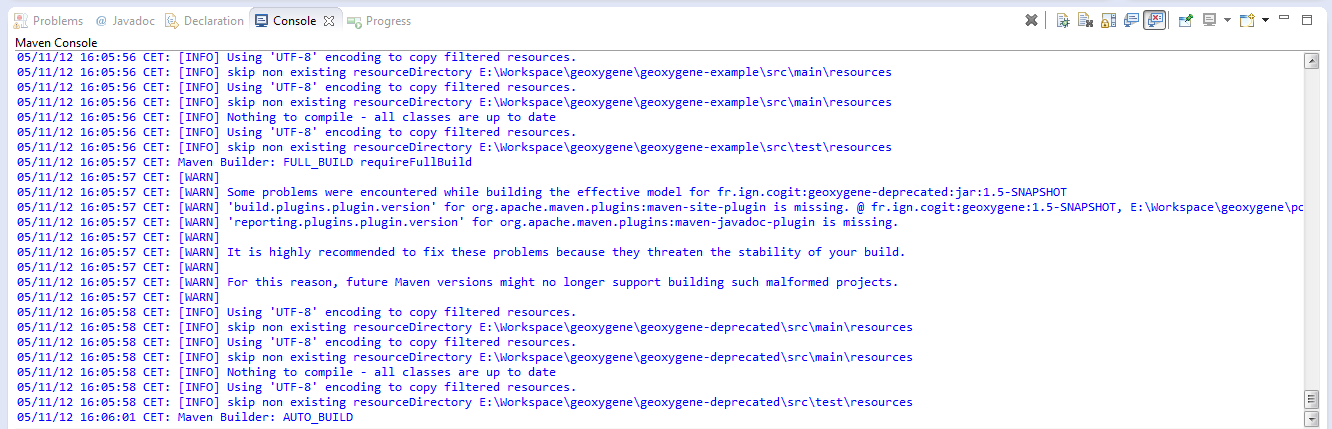
\includegraphics[width=0.5\linewidth]{../../resources/images/guide_installation/geoxygeneAutoBuild.png}
%\end{center}

\smallskip
 
%-------- cas 2
\begin{flushleft}
    \bf
    2ème cas : lancer un maven build manuellement.
\end{flushleft}

\noindent
Pour cela :\\

% 3 tableaux pour les 3 étapes
\begin{tabular}{p{6cm}l}
  {1. Sélectionner dans l'explorateur à droite, le projet "geoxygene". Puis dans le menu, cliquer sur Run $\Rightarrow$ Run Configurations.}&
   \imagetop{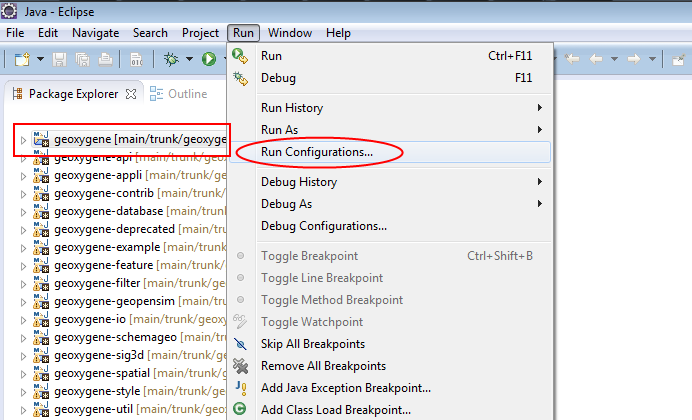
\includegraphics[width=0.45\textwidth]{../../resources/images/guide_installation/geoxygeneRunEtape1.png}} \\
\end{tabular}


\begin{tabular}{p{6cm}l}
   {2.  Sélectionner comme type de run "Maven", puis cliquer dans le menu en haut sur "New launch configuration"}&
   \imagetop{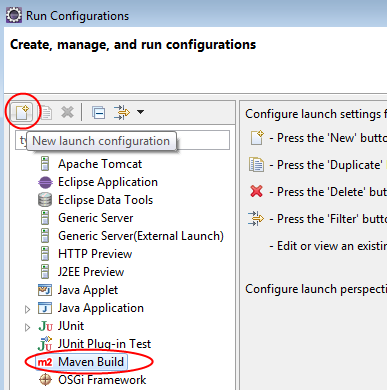
\includegraphics[width=0.4\textwidth]{../../resources/images/guide_installation/geoxygeneRunEtape2.png}} \\
\end{tabular}

\bigskip

\begin{tabular}{p{6cm}l}
   {3.  Dans la nouvelle fenêtre "Run configuration" configurer :
         \begin{enumerate}
         \item \emph{Name} : geoxygene
         \item \emph{Base directory} : saisir le chemin d'installation de GeOxygene (c'est celui de votre Workspace auquel il faut ajouter geoxygene)
         \item \emph{Goal} : clean install. Vous définissez la phase du cycle (clean, install, package, compile, test, site, ...)
         \item d'autres options peuvent être configurées dans cette interface si vous le souhaitez.
         \end{enumerate}}&
   \imagetop{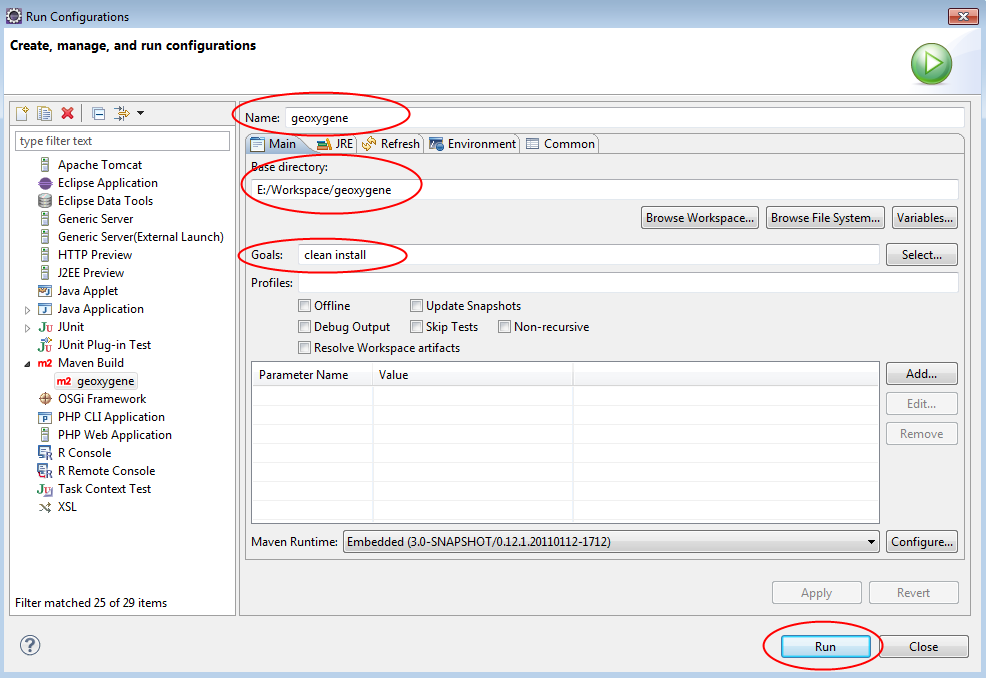
\includegraphics[width=0.55\textwidth]{../../resources/images/guide_installation/geoxygeneRunEtape3.png}} \\
 \end{tabular}





\bigskip
\noindent
Si tout se passe bien, Maven devrait récupérer tous les jars nécessaires et compiler le projet. 

%---------------------------------------------------------------------------------
\section{Exécution d'un exemple}
Une application exemple peut \^etre exécutée~: \emph{fr.ign.cogit.geoxygene.appli.GeOxygeneApplication}.

\bigskip

\noindent
Pour cela ouvrir le fichier GeOxygeneApplication.java qui se trouve dans le module : \\
\begin{tabular}[!t]{llll}
   geoxygene-appli $\Rightarrow$ src/main/java $\Rightarrow$  fr.ign.cogit.geoxygene $\Rightarrow$ appli
\end{tabular}

\bigskip

\noindent
Dans la fenêtre de l'éditeur de la classe, faire un click droit de la souris. Puis cliquer sur :\\
\begin{tabular}[!t]{llll}
"Run As" $\Rightarrow$ "Java Application"
\end{tabular}\\

\begin{center}
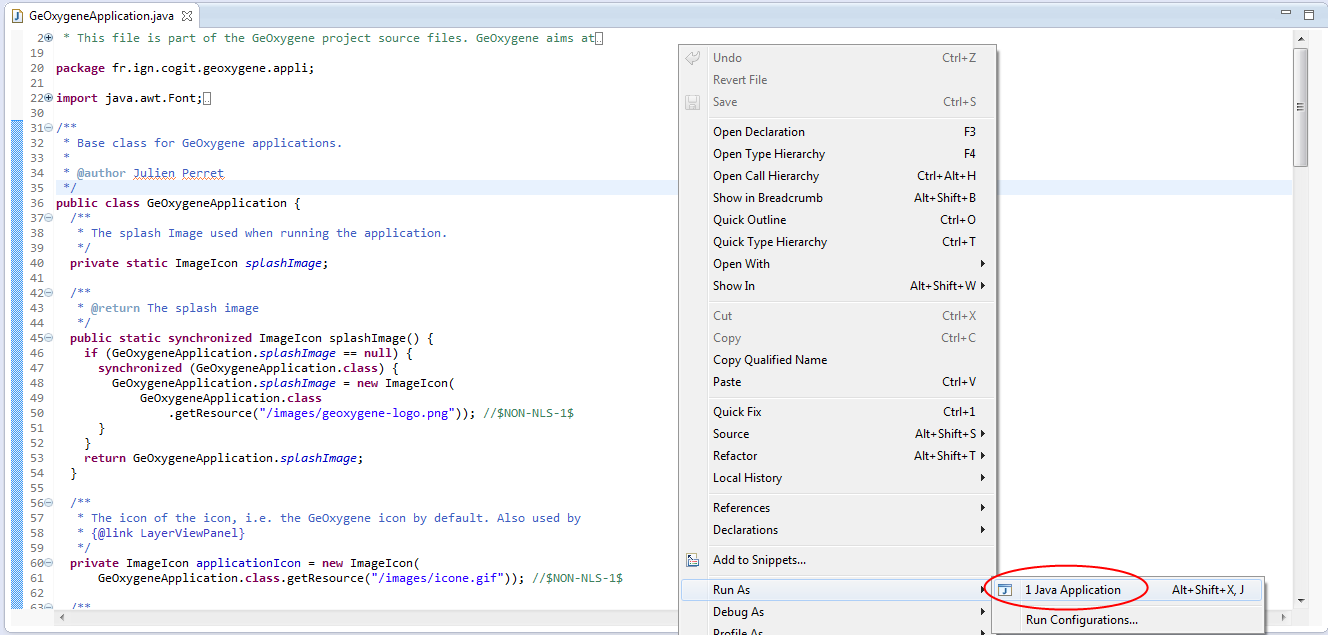
\includegraphics[width=0.5\linewidth]{../../resources/images/guide_installation/GeOxygeneAppliRunAs.png}
\end{center}

L'interface de GeOxygene est lancée !


%---------------------------------------------------------------------------------
\section{Configuration}


%-----
\subsection{Activation de la console Maven}

Ouvrir la fenêtre de la console en cliquant sur : {\emph{Window} $\Rightarrow$ \emph{Show View}  $\Rightarrow$ \emph{Console}}. Puis cliquer sur la petite flèche complètement à droite de la fenêtre "Open Console" et sélectionner "Maven Console" comme indiqué ci-dessous :

\begin{center}
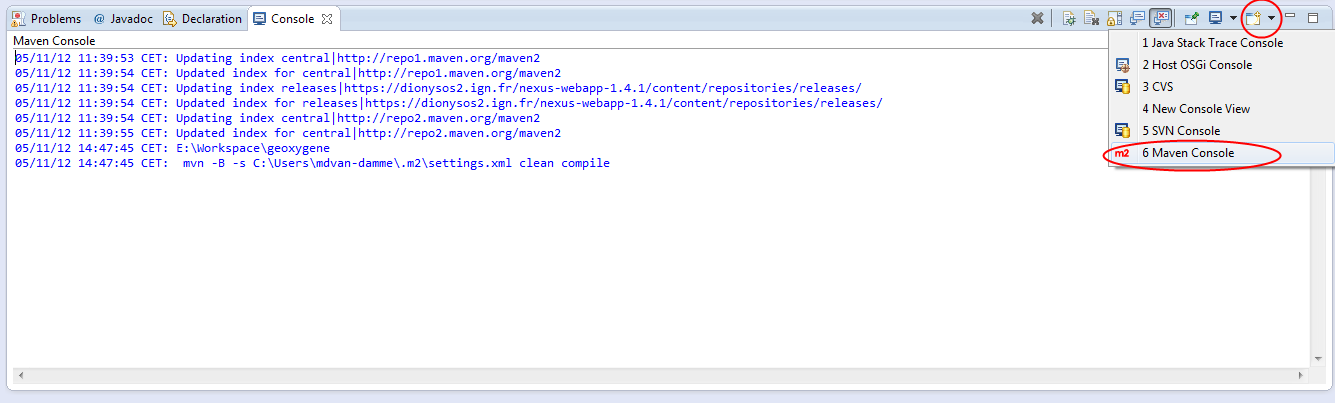
\includegraphics[width=0.5\linewidth]{../../resources/images/guide_installation/geoxygeneEtape5.png}
\end{center}

Il peut être utile de travailler avec la sortie de débogage Maven pour diagnostiquer les problèmes.




%---
\subsection{Convention de codage}

Parce qu'on passe plus de temps à lire du code qu’à en écrire, il faut configurer dans Eclipse la convention de programmation adoptée dans GeOxygène. Elle s'inspire avant tout de la convention de programmation recommandée pour tous les développements JAVA. Cette norme est dérivée de celle proposée par SUN à l’adresse :

\begin{tabular}[!t]{llll}
{\href{http://www.oracle.com/technetwork/java/codeconvtoc-136057.html}{http://www.oracle.com/technetwork/java/codeconvtoc-136057.html}}  
\end{tabular}

\noindent
Aller dans "Preferences $\Rightarrow$ Java $\Rightarrow$ Code Style $\Rightarrow$ Formatter" et cliquer sur "Import". 

\begin{center}
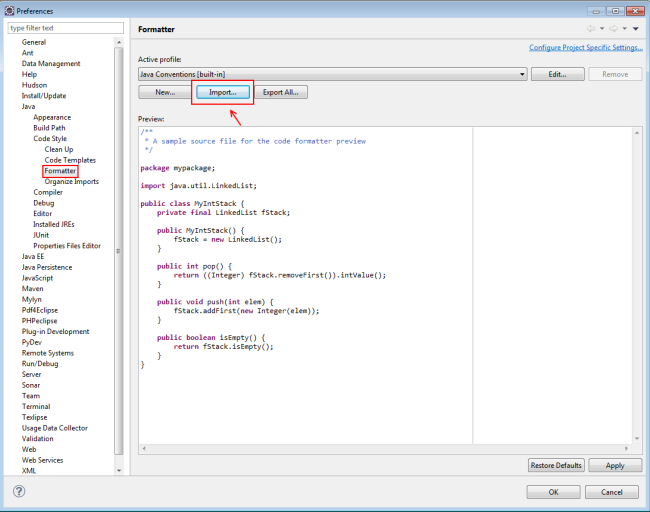
\includegraphics[width=0.5\linewidth]{../../resources/images/guide_installation/ConfigEclipseConventionCodage_1.png}
\end{center}

\noindent
Le template de la convention de nommage du COGIT «java\_cogit\_formatting\_conventions\_v1.xml» se trouve dans le code source du projet GeOxygene :

\begin{tabular}[!t]{llll}
geoxygene $\Rightarrow$  src $\Rightarrow$  main $\Rightarrow$  resources $\Rightarrow$  java\_cogit\_formatting\_conventions\_v1.xml
\end{tabular}

\smallskip

\noindent
Importer ce fichier et choisissez comme "Active profile" : "Java COGIT Formatting Conventions v1" 

\begin{center}
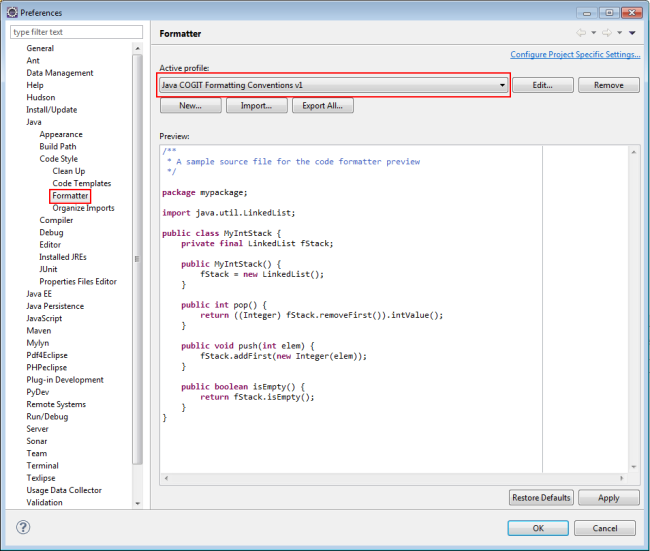
\includegraphics[width=0.5\linewidth]{../../resources/images/guide_installation/ConfigEclipseConventionCodage_2.png}
\end{center}


%---
%\subsection{Encodage}


%\subsection{ Accès aux bases de données}
%\subsection{Journalisation}






\end{document}
